\chapter{怎样验证这套实现}
\label{chap:validation}
\section{先检验数学身份，再检验求解能力}
软件会输出一个数字，不代表这个数字正确。本次验证分为四层：基础恒等关系和独立导数检查；受控合成数据恢复；公开实验强度的已知模型再精修；真实命令行与持久化 agent 的集成执行。它们回答不同问题，结果分别保存。

衍射导数使用另一路物理计算及中心差分检查，覆盖斜晶胞、反常散射、非对称平移群、特殊位置重根 ADP、占有率和约束以及多个孪晶畴。径向近端更新用独立的三次方程驻点计算检查全局最优；相位算法还检验原点协变、强度单位协变、Friedel 配对和保留集不泄漏。

像素压缩对任意结构预测与原始像素直接剖面比较，而不只在拟合最优点比较。这样可以确认后续结构搜索在整个可检查区域内看到同一个目标。共同像素结构精修同时检查恢复例和必然不可辨识的反演反例。

\section{从头求解的受控实验}
所有相位实验只提供晶胞、观测、不确定度和完整晶胞元素表，不提供真值原子坐标。恢复误差在允许原点、反演和同元素置换后计算。真值只用于产生数据和事后评价。

\begin{table}[tb]
\centering\small
\caption{本次合成盲解。每个场景四个起点全部得到可精修模型；表中 RMS 为代表结果，不能外推成实验成功率。}
\begin{tabularx}{\textwidth}{@{}Xrrr@{}}
\toprule 场景 & 观测数 & 负强度数 & 精修后 RMS / $\angstrom$\\\midrule
四碳，第一噪声档 & 4540 & 397 & 0.00106\\
四碳，第二噪声档 & 4540 & 868 & 0.00254\\
四碳，第三噪声档 & 4540 & 1298 & 0.00843\\
斜晶胞 O$_2$N$_2$C$_4$ & 4590 & 125 & 0.000997\\
\bottomrule
\end{tabularx}
\end{table}

四碳例使用四次起点、每次 400 轮，混合元素例为四次起点、每次 600 轮。结果说明带符号弱强度可以参与此求解机制；它们不是高无序 MOF、大晶胞或未知组成的验证集。

独立强度表的自动流程将 4540 条观测按关联分为 work 3406、selection 680、audit 454。四个起点产生候选后，选择并再精修一个模型；审计标准化残差 RMS 为 0.9653，坐标 RMS 为 $0.000979\angstrom$。该审计指标没有用于挑选起点。

\section{从混合观测组开始的自动流程}
合成双畴例有 2497 个高斯观测组，包括隔离、近重叠和完全重叠。work、selection、audit 分别为 1861、381、255 组。只用 work 中 1121 个隔离参考畴观测初始化相位，其中有 95 个负强度；它们仍然保留。

四个相位起点经过共同结构精修后均收敛。选择模型的晶畴比例约为 $(0.63237,0.36763)$，合成真值为 $(0.63,0.37)$；坐标 RMS 为 $0.002203\angstrom$，一次最终审计的模式标准化 RMS 为 1.02375。整个过程使用观测算子，没有把无法分离的分量当成独立测量。这是压缩高斯证据上的集成盲解，尚不是仪器原始帧重处理实验。
\begin{figure}[!htbp]
\centering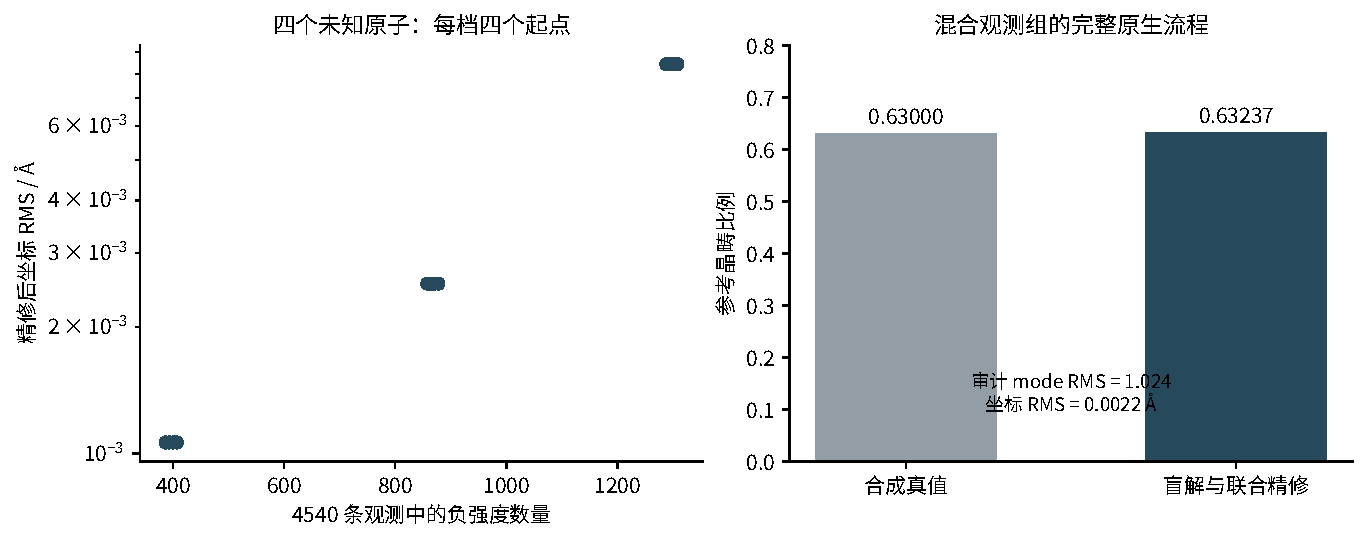
\includegraphics[width=\textwidth]{figures/09_blind_recovery.pdf}
\caption{左：三种噪声条件下的四起点盲解。横坐标仅描述数据，不用于裁掉负值。右：双畴混合观测流程恢复的比例与设定真值。数据来源为本次 \code{v08_phasing/result.json}。}
\end{figure}

\section{局部结构精修与不确定度}
对于 171 个区域、7011 个像素的三原子局部精修例，混合重叠和全部完全重叠两种设计都恢复了设定结构与 $(0.73,0.27)$ 的比例。全部重叠时，各区域信号秩为 1，但共享结构的 Jacobian 为 11/11。含噪声时参考畴比例为 0.7301858，条件标准不确定度为 0.0006302，最大坐标误差约 $0.003365\angstrom$。

最终 C++ 路径上，同一含噪数据的压缩目标与原像素背景剖面目标之差为 $-9.09\times10^{-13}$。若改成无反常散射的反演孪晶，结构 Jacobian 为 10/11，软件返回不可辨识的比例估计与空协方差。一个正确的求解器既要能恢复有信息的参数，也要识别没有信息的参数。

\section{实验数据回归：\texorpdfstring{FeN$_4$}{FeN4}}
公开数据来自 Bykov 等人的 FeN$_4$ 单晶研究及所存测量强度\cite{fen4}。本次读取 71 个实测 $F^2$ 与标准不确定度，从公开模型和一个扰动后的模型分别开始，使用原生散射和精修器；没有把文件中的计算结构因子当作观测，也没有调用 SHELXL 数值后端。

\begin{table}[tb]
\centering
\caption{FeN$_4$ 已知模型的实验强度再精修。此表验证一个给定模型的数值一致性，不评价从头求解。}
\begin{tabular}{@{}lrr@{}}
\toprule 指标 & 本次原生计算 & 公开参考值\\\midrule
$R_1\,[I>2\sigma(I)]$ & 0.040316 & 0.0403\\
$R_1$，全部观测 & 0.041268 & 0.0413\\
$wR_2$ & 0.081480 & 0.0815\\
拟合优度 & 1.183324 & 1.183\\
独立参数数 & 10 & 10\\
\bottomrule
\end{tabular}
\end{table}

使用的是同一个特定权重模型、各向同性位移参数和明确的特殊位置约束。良好一致性为原生内核提供实验数据支持，但一个样品不代表全部元素、消光、无序和孪晶功能已经等价。

\section{效率的测量范围}
\begin{table}[tb]
\centering\small
\begin{tabularx}{\textwidth}{@{}Xrr@{}}
\toprule 本机测量 & 基线 & 新路径\\\midrule
18 原子、1098 反射、70 参数精修中位时间 & 2.6817 s & 0.11729 s\\
同一精修的衍射前向调用数 & 988 & 7\\
3500\,$\times$\,64 SVD 例进程峰值 RSS & 260500 KiB & 81444 KiB\\
25 万像素增广 QR 的额外峰值分配 & 43.82 MB & 0.516 MB\\
该像素例的一次测量耗时 & 0.0215 s & 0.0595 s\\
\bottomrule
\end{tabularx}
\end{table}

精修时间比较明确使用同一 NumPy 缓存前向计算，区别是差分与解析导数；在本例中约快 22.9 倍，最终预测差在 $10^{-9}\sigma$ RMS 以下。C++ 与 NumPy 的同一解析模型比较另见第\ref{chap:kernels}章，不能把不同计时口径直接相乘。像素例比较的是预分配输入以外的额外分配，基线仅作稠密 QR，新路径还完成背景消元及信息分解。新路径在这一例中更省工作内存，但更慢；不能把内存比写成时间加速比。

记录环境为 Python 3.12.14、NumPy 2.3.5、SciPy 1.17.0、Gemmi 0.7.5。精修时间取三次单线程中位数；内存进程和像素分配实验各有明确口径，JSON 中保留原始数值。

\section{复现和下一批实验}
冻结源码后的完整回归包含 572 项通过的主测试，以及 136 个通过的子测试。还原侧为 366 项通过、11 项跳过；原生结构侧为 206 项通过、没有跳过，并启用了真实 MCP 标准输入输出测试。11 个跳过项需要当前环境没有安装的 DIALS、cctbx 或 dxtbx。C++ 数值测试和新增调度测试已经计入这些总数，不能重复相加。

完整相位、共同观测精修和 FeN$_4$ 回归又以明确指定的 C++ 后端生成了最终数值记录；前述差分与解析导数性能比较则明确指定 NumPy 后端。编译 wheel 与纯 Python wheel 另在独立目录检查实际导入和运行，使编译扩展缺失时的行为也有执行证据。

\begin{lstlisting}
python -m pytest tests tests_rebuild -q
ARIADNE_MCP_STDIO_TEST=1 python -m pytest native/tests -q
python benchmarks/v08_reduction.py
python native/validation/run_v08_refinement.py
python native/validation/run_v08_kernels.py
python native/validation/run_v08_joint.py
python native/validation/run_v08_phasing_autonomy.py
python native/validation/run_real_fen4.py
python docs/v08/tools/make_figures.py
\end{lstlisting}
测试应在两个独立 pytest 进程中运行，避免旧测试目录中同名模块和互相导入造成收集冲突。DIALS 相关测试只在具备真实原生运行环境时执行；本包的测试记录明确列出跳过项，不将它们计为通过。最终汇总见随包验证文件。

接下来最有价值的数据不是再增加一个容易的合成例，而是固定一批真实 MOF 原始帧：包括常规强衍射、不同弱信号比例、部分与完全重叠、溶剂无序和已知缺陷。应预先固定判断标准、外层扫描块划分和计算预算，比较反射预测残差、积分覆盖率、共同观测预测似然、结构误差和总运行资源。只有这些实验才能回答生产替代的范围。
